% !TeX program = lualatex
% ================================================================
% Polish Parallel Text Version of GeometryBasedStarters4Qs
%
% Generated by the server using the following settings:
%
%   language            Polish (pol)
%   text direction      left to right
%   font                Noto Serif
%   fallback font       Noto Serif
%   built from          latex/starters/retrieval/lessPriorKnowledge/geometryBasedStarters4Qs.tex
%   vocabulary key      latex/starters/retrieval/lessPriorKnowledge/geometryBasedStarters4Qs/L2/pol/geometryBasedStarters4Qs_polishKey.tex
%   tier 3 vocabulary   green   RGB 0 128 0
%   English text        black   RGB 0 0 0
%   Polish text         purple  RGB 112 48 160
%   layout macros       version 3
%
% Please don't edit any information in this comment block - the server
% compares it against the current settings and rebuilds this file when
% they differ, so changes here would be overwritten. However, feel free
% to make updates to the LaTeX below if you want to edit it.
% ================================================================

\documentclass[aspectratio=169]{beamer}
% ================================================================
% Copied from the English sheet this was translated from, so that
% anything it sets up for itself still works here
% ================================================================
\usepackage{amsmath}
\usepackage{tikz}
\usetikzlibrary{angles,quotes,calc}

% ================================================================
% Answer-overlay helpers
% ================================================================
\newcommand{\ablank}[1]{%
  \alt<2>{\textcolor{red}{#1}}{\underline{\phantom{#1}}}%
}
\newcommand{\ashow}[1]{\uncover<2->{\textcolor{red}{\small #1}}}
\newcommand{\ashowq}[1]{\alt<2->{\textcolor{red}{\small #1}}{?}}

% Answers drawn straight on to a TikZ diagram, revealed on overlay 2 like \ashow.
% Space is reserved on overlay 1, so the diagram does not move between slides.
\usetikzlibrary{overlay-beamer-styles}
\tikzset{
  ans/.style     = {red, thick, visible on=<2->},
  ansfill/.style = {red!15, visible on=<2->},
  anslab/.style  = {red, font=\tiny, visible on=<2->},
}

\title{Starter}
\author{}
\date{}

\setbeamertemplate{navigation symbols}{}

% Characters this language's font has not got are borrowed from another,
% rather than being silently dropped - see docs/translated-sheet-latex.md
\directlua{%
  if luaotfload and luaotfload.add_fallback then
    luaotfload.add_fallback("eallatinfallback",
      { "Noto Serif:mode=harf;" })
  else
    tex.error("this luaotfload is too old to register a fallback font")
  end
}
\usepackage[english]{babel}
\babelprovide[import]{polish}
\babelfont[polish]{rm}[Renderer=Harfbuzz, BoldFont={Noto Serif}, ItalicFont={Noto Serif}, BoldItalicFont={Noto Serif}, RawFeature={fallback=eallatinfallback}]{Noto Serif}
\babelfont[polish]{sf}[Renderer=Harfbuzz, BoldFont={Noto Serif}, ItalicFont={Noto Serif}, BoldItalicFont={Noto Serif}, RawFeature={fallback=eallatinfallback}]{Noto Serif}
\newcommand{\ealtext}[1]{\foreignlanguage{polish}{#1}}
\newcommand{\ealtextblock}[1]{{\raggedright\foreignlanguage{polish}{#1}\par}}
% ================================================================
% EAL layout helpers
% ================================================================
\usepackage{xcolor}

\definecolor{ealkeycolour}{RGB}{0,128,0}
\definecolor{ealenglish}{RGB}{0,0,0}
\definecolor{ealtwocolour}{RGB}{112,48,160}

\newsavebox{\ealboxen}
\newsavebox{\ealboxtr}
\newlength{\ealglosswd}
\newlength{\ealglossraise}
\setlength{\ealglossraise}{1.15em}

% a tier 3 word, in English and in translation alike
\newcommand{\ealkey}[1]{\textcolor{ealkeycolour}{#1}}
\newcommand{\ealkeytr}[1]{\textcolor{ealkeycolour}{\ealtext{#1}}}

% One translated word above one English word. Built from kernel
% primitives, never a tabular, which would break wherever the sheet
% loads array, booktabs or tabularx. The box is as wide as the wider of
% the two, so a long translation pushes its neighbours aside instead of
% overlapping them, and it claims its full height so a table row or a
% TikZ node makes room for it.
\newcommand{\ealgloss}[2]{%
  \sbox{\ealboxen}{\ealkey{#1}}%
  \sbox{\ealboxtr}{\small\textcolor{ealtwocolour}{\ealtext{#2}}}%
  \setlength{\ealglosswd}{\wd\ealboxen}%
  \ifdim\wd\ealboxtr>\ealglosswd\setlength{\ealglosswd}{\wd\ealboxtr}\fi
  \leavevmode
  \makebox[\ealglosswd][c]{%
    \makebox[0pt][c]{\usebox{\ealboxen}}%
    \makebox[0pt][c]{\raisebox{\ealglossraise}{\usebox{\ealboxtr}}}%
  }%
}

% opens up line spacing around a block of glosses, so the raised
% translations sit clear of the line above
\newenvironment{ealglossed}{\par\linespread{2.1}\selectfont\ignorespaces}{\par}

% a whole translated sentence above its English counterpart. block level,
% so it does not belong inside a tabular cell
\newcommand{\ealpara}[2]{%
  \par\addvspace{0.5\baselineskip}%
  {\color{ealtwocolour}\ealtextblock{#1}}%
  \penalty200
  {\color{ealenglish}#2\par}%
  \addvspace{0.5\baselineskip}%
}

\begin{document}

\begin{frame}
  \frametitle{Starter}

  \begin{columns}[t,onlytextwidth]
    % ===== LEFT COLUMN =====
    \begin{column}{0.52\textwidth}
      \textbf{1.}

      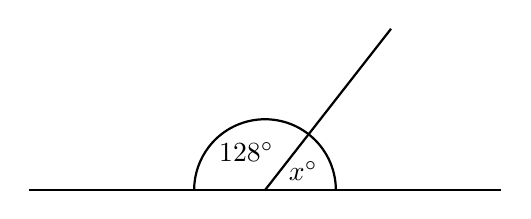
\begin{tikzpicture}[scale=1.0, thick]
        % Points
        \coordinate (A) at (0,0);
        \coordinate (L) at (-3,0);
        \coordinate (R) at (3,0);
        % A ray making 52 degrees with the rightward horizontal
        \path (A) -- ++(52:2.6) coordinate (C);

        % Line and ray
        \draw (L) -- (R);
        \draw (A) -- (C);

        % Angle marks
        % Obtuse angle on the left (128°)
        \pic[draw,angle radius=9mm,"$128^\circ$" {scale=1}] {angle = C--A--L};

        % Acute angle on the right (x°)
        \pic[draw,angle radius=9mm,"$x^\circ$" {scale=1}] {angle = R--A--C};
      \end{tikzpicture}

      \vspace{0.7em}
      \ealpara{Znajdź \ealkeytr{wartość} $x$.}{Find the \ealkey{value} of $x$.}
      \ashow{\quad $x = 52^\circ$}

      % ---- Flexible space to push #3 down to align with #4 ----
      \vfill
      \vspace{4em}

      \textbf{3.} \quad $372 + 458 = \ablank{830}$
    \end{column}

    % ===== RIGHT COLUMN =====
    \begin{column}{0.48\textwidth}
      \textbf{2.}

      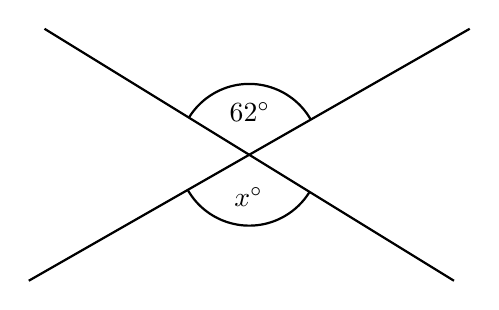
\begin{tikzpicture}[scale=1.0, thick]
        % Intersection point
        \coordinate (O) at (0,0);

        % Two intersecting lines
        \coordinate (A1) at (-2.8,-1.6);
        \coordinate (B1) at (2.8,1.6);
        \coordinate (C1) at (-2.6,1.6);
        \coordinate (D1) at (2.6,-1.6);
        \draw (A1) -- (B1);
        \draw (C1) -- (D1);

        % Mark the top angle as 62°
        \pic[draw,angle radius=9mm,"$62^\circ$" {scale=1}] {angle = B1--O--C1};

        % Mark the vertically opposite (bottom) angle as x°
        \pic[draw,angle radius=9mm,"$x^\circ$" {scale=1}] {angle = A1--O--D1};
      \end{tikzpicture}

      \vspace{0.7em}
      \ealpara{Znajdź \ealkeytr{wartość} $x$.}{Find the \ealkey{value} of $x$.}
      \ashow{\quad $x = 62^\circ$}

      % ---- Flexible space to push #4 down to align with #3 ----
      \vfill
      \vspace{1em}
      \textbf{4.} \quad $(84 \div 6) \times 3 = \ablank{42}$
    \end{column}
  \end{columns}

\end{frame}

% --- Optional: Answers slide ---
% \begin{frame}
%   \frametitle{Answers}
%   \begin{enumerate}
%     \item $x = 52^\circ$ \hfill (angles on a straight line sum to $180^\circ$)
%     \item $x = 62^\circ$ \hfill (vertically opposite angles are equal)
%     \item $372 + 458 = 830$
%     \item $84 \div 6 \times 3 = 14 \times 3 = 42$
%   \end{enumerate}
% \end{frame}

\end{document}